\documentclass[12pt]{article}
\usepackage{graphicx}
\usepackage[utf8]{inputenc}
\usepackage[ngerman]{babel}
\usepackage[T1]{fontenc} 
\usepackage{wrapfig}
\usepackage{multirow}
\usepackage[a4paper, left=3cm, right=2.5cm, top=2.5cm]{geometry}
\usepackage[onehalfspacing]{setspace}


\begin{document}

\begin{titlepage}
\newcommand{\HRule}{\rule{\linewidth}{0.5mm}}
\center

\textsc{\LARGE Hochschule Kempten}\\[0.5cm]
\textsc{\large Fakultät Informatik}\\[0.5cm]
\textsc{\large Masterstudiengang Angewandte Informatik}\\[1.5cm]

\HRule \\[0.4cm]
{\huge \bfseries Verhaltensausbreitung}\\[0.2cm]
\HRule \\[1.0cm]

\textsc{\LARGE Seminararbeit}\\[0.5cm]
\textsc{\large im Seminar}\\[0.5cm]
\textsc{\LARGE Informationssuche, Soziale Netzwerke, Moderne Algorithmen}\\[1.5cm]



\begin{minipage}{0.4\textwidth}
\begin{flushleft}\large
\emph{Autor:}\\
Fabian Thomas \textsc{Schafroth}
\end{flushleft}
\end{minipage}
~
\begin{minipage}{0.4\textwidth}
\begin{flushright}\large
\emph{Betreuer:}\\
Prof. Dr. Jochen \textsc{Staudacher}
\end{flushright}
\end{minipage}\\[4cm]
{\large \today}\\[3cm]

%includegraphics{logo}\\[1.0cm]

\vfill
\end{titlepage}
\newpage
	\pagenumbering{roman}
	\tableofcontents
\newpage
\pagenumbering{arabic}

\section{Einführung}
Das Aufkommen von neuen Verhaltensweisen und deren Verbreitung in sozialen Netzen sind Phänomene, die sowohl in tierischen als auch in menschlichen Gemeinschaften beobachtet werden können und von wissenschaftlichem Interesse sind. Ein Individuum innerhalb einer Gemeinschaft ist unter normalen Umständen stets bestrebt, sich den Normen und Verhaltensweisen der Mehrheit anzupassen. Dieses Verhalten lässt sich damit begründen, dass homogene Gemeinschaften besonders gut funktionieren. Solche Gemeinschaften unterscheiden sich von heterogenen besonders darin, dass sie sich aus Individuen zusammensetzen, welche große Übereinstimmungen in ihrer Art, Sprache und dem Verhalten aufweisen \cite{Rogers03}. Diese homogenen Individuen halten einen engen Kontakt zueinander, tauschen sich oft aus und schätzen die jeweilige Meinung ihrer nächsten Bekannten. Zudem werden vertraute Personen im nahen sozialen Umfeld bereitwilliger als Vorbilder akzeptiert als fremde Menschen.\\\\
Die auf diese Situation aufbauende Theorie der Verhaltensausbreitung geht als Grundlage davon aus, dass ein Individuum stets sein nahes soziales Umfeld betrachtet und Veränderungen darin wahrnimmt, sowie sie gegebenenfalls auf ihren Nutzen hin analysiert. Sollte sich in diesem Umfeld eine Änderung in der Verhaltensweise vollzogen haben, wird das Individuum früher oder später nachziehen, sofern es einen tatsächlichen (oder auch nur gefühlten) Vorteil darin sieht. Was mit der Einführung eines neuen Verhaltens hier konkret gemeint ist, kann vielfältig sein. Die Verwendung einer neuen Technologie zum Ackerbau, ein neuer Kleidungsstil oder ein schnellerer Web Browser.\\\\
Der Beginn einer jeden Verhaltensausbreitung beginnt folglich damit, dass ein oder mehrere Individuen aus eigenen Stücken, ohne Einfluss durch ihr nahes soziales Umfeld, ein neues Verhalten annehmen. Von diesen Pionieren ausgehend kann sich dieses Verhalten innerhalb der Gemeinschaft durch die zuvor bereits genannten, engen Beziehungen verbreiten. Dieser Vorgang wird als Kaskade bezeichnet, eine Ausbreitung ähnlich einer Kettenreaktion. Ihr endgültiges Ziel ist dann erreicht, wenn alle Individuen einer Gemeinschaft, das durch die Kaskade verbreitete, neue Verhalten angenommen haben.
Kaskaden lassen sich bezüglich mehrerer Faktoren auf ihren Erfolg hin analysieren.
\begin{enumerate}
\item Wie schnell verbreitet sich eine Kaskade.
\item Was für Bedingungen sind für die Verbreitung von Bedeutung.
\item Gibt es innerhalb von sozialen Netzwerken natürliche Hindernisse für die Verhaltensausbreitung.
\item Gelingt es einer Innovation eine vollständige Kaskade herbeizuführen.
\end{enumerate}
Besonders interessant sind Kaskaden und ihre Effekte für das moderne Marketing, da man möglichst akkurate Modelle erstellen möchte, um neue Produkte am Markt bestmöglich zu verbreiten oder künstliche Trends zu setzen. Eine gänzlich neue Dimension haben in diesem Bereich die Internetmedien und darin entstandenen online Netzwerke geschaffen.\\\\



\section{Verhaltensausbreitung}
Nach Rogers lässt sich die Verhaltensausbreitung auf vier übergeordnete Aspekte konzentrieren. Die Innovation, welche neu in einem sozialen Netzwerk angekommen ist. Die Kommunikationskanäle, welche innerhalb dieses Netzwerkes bestehen und damit auch das soziale Gefüge definieren. Die Personen welche die Kanäle zueinander unterhalten. Sowie die Zeit, welche in mehreren Blickwinkeln maßgeblich den Erfolg einer Verhaltensausbreitung definiert. Die in diesem Kapitel folgenden Ausführungen über die soziologischen Grundlagen der Verhaltensausbreitung, orientieren sich eng an den Inhalten von Everett Rogers Buch "`Diffusion of Innovation"' \cite{Rogers03}
\subsection{Innovation}
Als Innovation wird gemeinhin ein neues Verhalten bezeichnet, welches von den Mitgliedern eines sozialen Netzwerkes entweder adaptiert oder abgelehnt werden kann. Für welche der beiden Wahlmöglichkeiten sich die Individuen entscheiden, hängt im Rahmen der Betrachtung von Kaskaden maßgeblich davon ab, wie viele benachbarte Kontakte sich bereits für das neue Verhalten entschlossen haben. Entgegen diesem rein analytischen Ansatz beschäftigt sich dieser Abschnitt detaillierter mit den soziologischen Faktoren, warum eine Innovation Erfolg hat oder nicht.\\\\
Rogers definiert fünf Attribute, welche mit unterschiedlicher Gewichtung dazu beitragen, ob die Kaskade einer Innovation sich über ein gesamtes Netzwerk verbreiten kann.
\begin{enumerate}
\item \textbf{Relativer Vorteil}\\ Als relativer Vorteil einer Innovation lässt sich das Gefühl umschreiben, nach welchem die Individuen eines sozialen Netzwerks einen Vorteil für sich darin sehen, ein neues Verhalten zu adaptieren. Es wird dabei großen Wert auf die Tatsache gelegt, dass es nicht nötig ist, dass die Innovation einen tatsächlich quantitativ oder empirisch erfassbaren Vorteil bringt. Denn nicht zwangsläufig setzt sich immer das beste Verhalten durch. Beispiele aus der Realität gibt es hierfür zahlreiche\footnote{Das JPEG2000 Bildformat welches dem universal verbreiteten JPEG überlegen ist. Das DVORAK-Tastaturlayout welches, anders als das QWERTY-Layout, nicht entwickelt wurde um Schreibmaschinenschreiber auszubremsen.}
\item \textbf{Kompatibilität}\\ Die Kompatibilität einer Innovation bestimmt, wie gut die Innovation mit dem vorherrschenden Normen und Wertesystem einer Gemeinschaft im Einklang ist. Je gegenläufiger diese beiden Konzepte zu einer möglichen Innovation sind, desto schwerer wird sie es haben, sich innerhalb der homogenen Gemeinschaft durchzusetzen.
\item \textbf{Komplexität}\\ Die Komplexität einer Innovation beschreibt, wie schwierig es für ein Individuum ist sie zu adaptieren. Hieraus lässt sich leicht der Schluss ziehen, je einfacher zu verstehen eine Innovation ist, desto schneller werden viele Menschen sie adaptieren. Smartphones sind das Paradebeispiel für eine neue Technologie, die einen phänomenalen Erfolg vorweisen kann, hauptsächlich aufgrund der einfachen Bedienbarkeit.
\item \textbf{Erprobbarkeit} \\ Am Klassischen Beispiel der Verbreitung von Hybriden Mais-Samen unter Bauern in Iowa (Siehe Kapitel \ref{ss_history}) lässt sich erkennen, welche Bedeutung die Erprobbarkeit einer Innovation hat. Kaum einer der Bauern hätte sich für die neuen Samen entschlossen, wenn er von einem Tag auf den anderen mit seinem kompletten Anbaugebiet auf die neuen Samen hätte wechseln müssen. Stattdessen testeten die meisten Bauern die neuen Samen erst auf einem kleinen Teil ihres Ackers und als dieser gute Erträge abwarf, wechselten sie dann komplett. Konkret bedeutet dies, je unverbindlicher die Adaption eines neuen Verhaltens ist, desto eher sind die Menschen bereit diesen Schritt zu wagen.
\item \textbf{Beobachtbarkeit} \\ Individuen tauschen sich innerhalb eines engen sozialen Netzwerkes nicht nur verbal aus, sondern beobachten sich auch gegenseitig. Daher ist es für eine Innovation besonders nützlich, wenn ihr (vermeintlich oder tatsächlicher) Vorteil gut sichtbar für jeden ist. Das Prinzip der Beobachtbarkeit ist maßgeblich für das im Kapitel \ref{s_verhaltenmodel} vorgestellte Modell der Verhaltensausbreitung. Ein Individuum wechselt dann hin zu einem neuen Verhalten, wenn es jenes bei einem bestimmten Anteil seiner unmittelbaren Nachbarn beobachten kann.
\end{enumerate}
\subsection{Das soziale Netzwerk}

\begin{figure}
  \begin{center}
    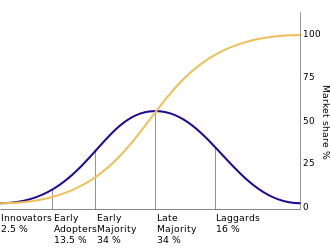
\includegraphics[width=0.80\textwidth]{pic_diffusion.png}
      \caption{Zusammenspiel zwischen Personentypen und Innovation} 
  Quelle: Wikipedia
  \end{center}
  \label{pic_diffusion}
\end{figure}

Neben den im vorherigen Abschnitt beschrieben Qualitäten, welche eine Innovation besitzt um ihre Verbreitung zu begünstigen, ist auch die Struktur des sozialen Netzwerkes von großer Bedeutung. Allgemein formuliert besteht das Gebilde eines sozialen Netzwerks aus den Personen welche es bevölkern und den Bekanntschaften welche sie untereinander haben. Manche Personen sind eher bereit eine Neuerung zu akzeptieren als andere. Ebenso haben manche Bekanntschaften höheren Einfluss auf ein Individuum als andere. Im Weiteren Verlauf dieses Abschnitts werden die wichtigsten Personengruppen sowie Verbindungstypen erläutert.

\subsubsection{Personen}
Die für die Verhaltensausbreitung relevanten Personen eines sozialen Gefüges lassen sich in fünf Kategorien unterteilen, welche durch die Zeit, die sie brauchen um eine neue Innovation zu akzeptieren, definiert werden. \cite{Rogers03}
\begin{enumerate}
\item \textbf{Innovatoren}: Innovatoren sind die ersten Personen innerhalb eines sozialen Netzwerkes, welche sich einer neuen Innovation annehmen und sie adaptieren. Diese Personen haben meist eine herausragende soziale oder intellektuelle Stellung innerhalb einer Gemeinschaft. Ihre Beziehungen reichen über sogenannte Weak Ties (Siehe Kap. \ref{intro_ties}) weit über das unmittelbare soziale Netz hinaus. Somit erfahren sie früher als andere von neuen Innovationen. Die initiale Adaption eines neuen Verhaltens durch einen Innovator markiert auf der Zeitlinie den Zeitpunkt $t_0$.
\item \textbf{Frühzeitige Anwender}: Diese Personengruppe hat meist einen direkten Kontakt zu den Innovatoren und ist somit prädestiniert, ein Verhalten sehr früh in der Zeitlinie einer Verhaltensausbreitung zu adaptieren. Der größte Unterschied zwischen den frühzeitigen Anwendern und den Innovatoren ist, dass sie bereits durch Observation innerhalb ihres sozialen Umfeldes sich zum Verhaltenswechsel entschlossen haben.
\item \textbf{Frühe und späte Mehrheit}: Diese beiden Klassen zusammen sind im Konzept der Personen eines sozialen Netzwerks mit Abstand die größte Gruppe. Die Unterscheidung zwischen früher und später Mehrheit ist rein zeitlicher Natur, da zwischen den Mitgliedern dieser Gruppe untereinander kein bemerkenswerter sozialer oder gesellschaftlicher Unterschied besteht. Auch sie lassen sich durch ihr unmittelbares soziales Umfeld beeinflussen und werden adaptieren wenn für sie ihr persönlicher Nutzen einer Adaption groß genug erscheint.
\item \textbf{Nachzügler}: Nachzügler stehen am Ende der Kette und adaptieren ein neues Verhalten erst dann, wenn fast schon das gesamte soziale Netz hin zu dieser Innovation gewechselt ist. Sie besitzen innerhalb einer Gesellschaft häufig einen niederen Stand oder verfügen über wenige soziale Verknüpfungen, sowie eine geringe Innovationsbereitschaft. Unter realen Bedingungen kommt es selten vor, dass eine Innovation ein gesamtes soziales Netz vollständig gewinnen kann. Meist bleiben immer Personen übrig, welche entgegen aller Vorteile an älteren Verhalten festhalten. Diese würden jedoch, da sie eine gegebene Innovation nie adaptieren, eine eigene Gruppe bilden. Denn der Begriff Nachzügler impliziert, dass spätestens zu einem Zeitpunkt $t_x >> t_0$, wenn auch spät, trotzdem adaptiert wird.
\end{enumerate}
\subsubsection{Kanäle der Verhaltensausbreitung}
\label{intro_ties}
Damit ein Individuum überhaupt auf die Idee kommt sein momentanes Verhalten durch ein neues zu ersetzen, muss als grundsätzliche Annahme gegeben sein, dass das Individuum von diesem neuen Verhalten über einen seiner Sinne Kenntnis genommen hat. Entweder er hat die Vorzüge des neuen Verhaltens selbst gesehen oder von einem Freund, beziehungsweise aus den Nachrichten davon gehört. Die Kanäle über welche sich die Information über eine neue Innovation verbreiten, sind so vielfältig, dass es den Rahmen dieser Arbeit sprengen würde, sie im Detail zu benennen \cite{strang98}. Allerdings bietet sich die nähere Analyse von zwei Obergruppen an, über welche sich Informationen in sozialen Gemeinschaften verbreiten.
\paragraph{Strong Ties}
Unter Strong Ties (Starke Verknüpfungen) wird in einer Gemeinschaft die unmittelbare soziale Umgebung eines Individuums definiert. Diese besteht aus sehr nahen Verwandten, Bekannten und Freunden. Zu ihnen hat das Individuum eine sehr enge Verknüpfung, es schätzt ihre Meinung und meistens teilt es auch Verhaltensweisen sowie Interessen. Dies ergibt sich aus dem natürlichen Bestreben eines Individuums, sich mit Personen zu umgeben die ihm ähnlich sind\cite{strang98}. Strong Ties spielen bei der Verhaltensausbreitung die beherrschende Rolle, da hauptsächlich über sie die Verbreitung einer Innovation stattfindet. Es hat deutlich mehr Gewicht für ein Individuum, wenn einer seiner besten Freunde ein neues Verhalten adaptiert, als wenn es ein flüchtiger Bekannter tut. Während die Strong Ties folglich sehr förderlich für die Verhaltensausbreitung sind, so haben sie einen großen Nachteil was die pure Informationsverbreitung betrifft. Gerade weil die soziale Struktur innerhalb eines Netzwerks aus Strong Ties stark verknüpft ist, gibt es darin wenig neue Information. Die Informationen welche ein Individuum von einem besten Freund oder nahem Verwandten bekommen kann, besitzt es in vielen Fällen schon.
\paragraph{Weak Ties}
Das im Punkt zu den Strong Ties angesprochene Problem über den Mangel an neuen Informationen in eng verknüpften sozialen Netzwerken, wird durch Weak Ties (schwache Verknüpfungen) gelöst. Diese sind Verbindungen zwischen zwei Personen welche sich selbst nicht zu ihrem unmittelbaren Bekanntenkreis zählen würden. Oft bilden diese Verknüpfungen somit Brücken zwischen zwei hauptsächlich aus Strong Ties bestehenden Netzwerkteilen. Veranschaulichen lässt sie dies beispielsweise mit zwei Dörfern. Innerhalb der Dörfer kennen sich die Menschen gut und haben ein eng verknüpftes soziales Netzwerk untereinander. Zum anderen Dorf jedoch bestehen nur wenige Verbindungen. Vielleicht kennt der ein oder andere jemand aus dem jeweils anderen Dorf, aber bei weitem nicht so gut wie seine unmittelbaren Mitbewohner. Über solche Kanäle wird keine Verhaltensausbreitung entstehen, da sie dafür nicht stark genug sind. Wohl allerdings lässt sich über diesen Weg die Information über ein neues Verhalten verbreiten. Strang und Soule \cite{strang98} nennen in ihrer Arbeit das Beispiel von Vorstandsmitgliedern, die in mehreren Unternehmen in den Vorständen sitzen, um somit von neuen Strategien zu erfahren. Diese werden dann in ihren eigenen Unternehmen den Entscheidungsträgern vorgestellt und können von ihnen adaptiert werden.
\subsection{Zeit als Faktor}
Die Zeit als Faktor findet sich in drei Bereichen einer Verhaltensausbreitung wieder.
\begin{enumerate}
\item Der Entscheidungsfindungsprozess durchläuft entlang der Zeitachse mehrere Stufen, in welchen sich das Individuum vom erstmaligen Hören einer Innovation bis hin zu dessen Adaption vorarbeitet. Wie schnell dies geschieht ist abhängig von den sozialen Strukturen und der Einstellung der Person selbst.
\item In welches Spektrum der Personen ein Individuum zuzuordnen ist hängt maßgeblich davon ab, wann es sich dazu entscheidet eine Innovation anzunehmen. Während Innovatoren den Startschuss setzen entschließen Nachzügler sich erst sehr spät im Prozess der Verhaltensausbreitung eine Adaption in Betracht zu ziehen.
\item Der dritte Faktor ist definiert als die Rate der Adaption, welche sich durch die Anzahl der Individuen berechnet, die in einem gegebenen Zeitintervall ein neues Verhalten angenommen haben.
\end{enumerate}

\subsection{Beispiele}
\label{ss_history}
Eine der ersten Studien zum Thema Verhaltensausbreitung wurde von Bryce Ryan und Neil Gross im US-Bundesstaat Iowa durchgeführt. Dieser im Midwesten der USA gelegene Staat, ist besonders geprägt durch die dort vorherrschende Landwirtschaft speziell dem Anbau von Mais. In ihrer Studie "Acceptance and Diffusion of Hybrid Corn Seed in two Iowa Communities" \cite{Ryan43} untersuchten Ryan und Gross wie, warum und über welche Wege ein neu entwickelter, bezüglich des Ertrags besserer, Hybridsamen Verbreitung fand. Dazu befragten sie mehrere Bauern wann sie damit begonnen hätten das neue Saatgut zu verwenden und wer sie auf die Idee dazu gebracht hatte. Ein Kernergebnis der Studie war, dass viele der Bauern bereits lange vor ihrer eigenen Adaption des neuen Saatguts, von seiner Existenz erfahren hatten. In den meisten Fällen durch Verkäufer, welche natürlich versuchten das neue Produkt in den Markt einzuführen. Jedoch überzeugen ließen sich die meisten der Bauern erst zu dem Zeitpunkt, als ein bekannter oder benachbarter Bauer den Hybridsamen erfolgreich einsetzte. Dies ist ein exemplarischer Fall für die Unterschiede zwischen Strong und Weak Ties. Über die Weak Ties (in diesem Fall die Verkäufer) trug sich lediglich die Information in das Netzwerk, allerdings nicht die Verhaltensausbreitung. Diese fand über die Mundpropaganda mit Bekannten und Nachbarn statt (Strong Ties). \\\\
Ein weiteres Beispiel welches Everett Rogers in seinem Buch Diffusion of Innovation beschreibt, handelt von einem peruanischen Dorf, in welchem die Regierung mittels eines Programms versuchen wollte, die Bewohner dazu zu bringen ihr Trinkwasser vor dem Konsum abzukochen. Viele Krankheitsfälle die eindeutig auf verschmutztes Trinkwasser zurückzuführen waren, ließen die Regierung diese Maßnahme ergreifen. Dazu wurde in die Gemeinschaft eine Frau des Gesundheitsministeriums geschickt, welche die ortsansässigen Hausfrauen schulen sollte. Das Projekt scheiterte nach mehreren Monaten damit, dass kaum Haushalte im Dorf das neue Verhalten angenommen hatten. Die Problematik hier lässt sich mit einer fehlenden Kompatibilität erklären. Die Einwohner haben ein traditionelles Verständnis vom Konsum von heißen und kalten Getränken. Das Bild hierbei ist, dass nur kranke Menschen heiße Getränke zu sich nehmen. Somit stieß die Idee, als gesunder Mensch heißes (oder eigentlich nur zuvor abgekochtes) Wasser zu trinken auf massiven Widerstand, da sie den herrschenden Normen nicht entsprach. \\\\
Ein aktuelleres Beispiel einer gescheiterten Verhaltensausbreitung wegen mangelnder Kompatibilität, ist der Versuch der Umweltpartei "`Bündnis 90 die Grünen"' einen sogenannten "`Veggi-Day"' in staatlichen Kantinen einzuführen. Das Thema im Wahlkampf 2013 dabei war, dass es in diesen Kantinen an einem Tag in der Woche nur vegetarisches Essen geben sollte. Wenngleich es sich dabei lediglich um eine Idee gehandelt hatte, welche nur auf einen sehr kleinen Teil der Bevölkerung eine Auswirkung gehabt hätte, wurde sie sofort massiv abgelehnt und die Partei bei der folgenden Wahl abgestraft. 

\section{Modellierung eines soziale Netzwerks}
Um die im vorherigen Abschnitt dargestellten, vielschichtigen Aspekte eines realistischen sozialen Netzwerks für Analysezwecke zu verwenden, ist eine gewisse Abstraktion notwendig. Die Grundannahme besteht darin, dass jedes soziale Netzwerk ein Gebilde ist aus Personen, Verbindungen zwischen diesen Personen und Verhalten welche von ihnen angenommen werden können. Eine dafür sehr gut geeignete Repräsentation ist ein Graph, dessen Knoten als Personen und Kanten als Verbindungen dienen. Die verschiedenen Verhaltensweisen können als Attribute der Knoten interpretiert werden.\\\\
\begin{figure}
  \begin{center}
    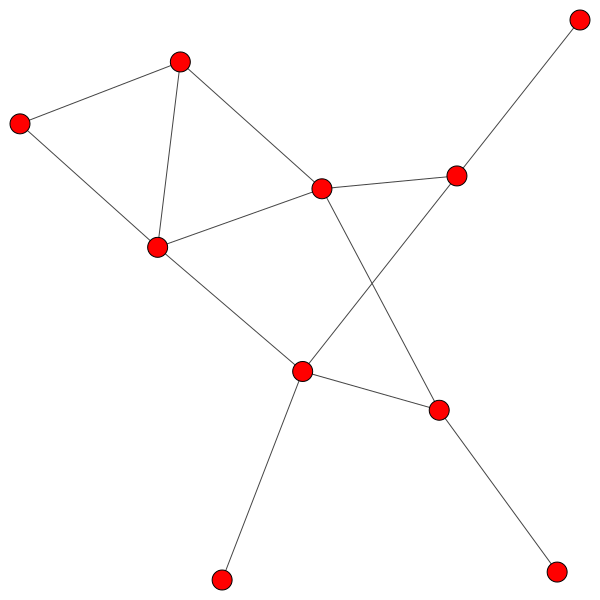
\includegraphics[width=0.60\textwidth]{pic_simpleGraph.png}
    \label{pic_simpleGraph}
  \end{center}
  \caption{Ein einfacher, den Bedingungen entsprechender Graph}
\end{figure}Jedoch ist nicht jeder Graph automatisch geeignet um ein soziales Netzwerk, besonders im Bezug auf die Verhaltensausbreitung, zu repräsentieren. Die hierfür verwendeten Graphen müssen nach Morris \cite{morris98} einer Reihe von grundlegenden Eigenschaften entsprechen (siehe Abb. \ref{pic_simpleGraph}) .
\begin{enumerate}
\label{enum_graphConditions}
\item Der Graph muss zusammenhängend sein. Dies bedeutet, dass von jedem beliebigen Knoten des Graphen aus, jeder beliebige andere Knoten über einen aus Kanten bestehenden Weg erreicht werden kann. Man darf unter dieser Bedingung die Tatsache verstehen, dass jeder Mensch auf der Welt, über eine endliche Anzahl an Verbindungen, mit jedem anderen Menschen verknüpft ist. Studien zum Thema des "`Small-World-Phenomena"' beschäftigen sich weiterführend mit dieser These (\cite{Easly10} Kapitel 20).
\item Der Graph muss ungerichtet sein. Diese Bedingung setzt als Grundlage voraus, dass wenn ein Individuum A das Individuum B kennt, B ebenfalls der Existenz von A gewahr ist. Dies entspricht nicht immer exakt den reellen Bedingungen (Stalker, Prominente), ist aber für die Analyse solcher Netzwerke hinreichend annehmbar.
\item Der Graph muss die Eigenschaft der Irreflexivität besitzen. Angewandt auf die Analyse sozialer Netzwerke versteht man darunter, dass kein Knoten sein eigener Nachbar ist. Das heißt, kein Individuum beeinflusst sich selbst bei seiner Entscheidung hin zu einem neuen Verhalten. 
\item Die Bedingung der Symmetrie betont, dass wenn ein Knoten A der Nachbar von Knoten B ist, so ist auch B ein Nachbar von A.
\end{enumerate}


\subsection{Weak- und Strong Ties}
Wie im Kapitel \ref{intro_ties} bereits dargelegt, gibt es mit Strong- und Weak Ties zwei Obergruppen, in welche sich sämtliche Verbindungen innerhalb eines Netzwerks klassifizieren lassen. Abbildung \ref{pic_ties} zeigt ein typisches, einfaches Beispiel für einen Graph mit klar erkennbaren Strong- und Weak Ties (starke Kanten sind Rot markiert und schwache Blau).\\
Klar identifizierbar sind hierbei die beiden eng verbundenen Gemeinschaften, welche untereinander Strong Ties unterhalten. Hinüber zur jeweils anderen Gemeinschaft existiert nur ein einzelner Weak Tie. Dieser wird niemals effektiv für die Verhaltensausbreitung dienen, aber potentiell die Information über neue Verhalten zwischen den Gemeinschaften transportieren.

\begin{figure}
  \begin{center}
    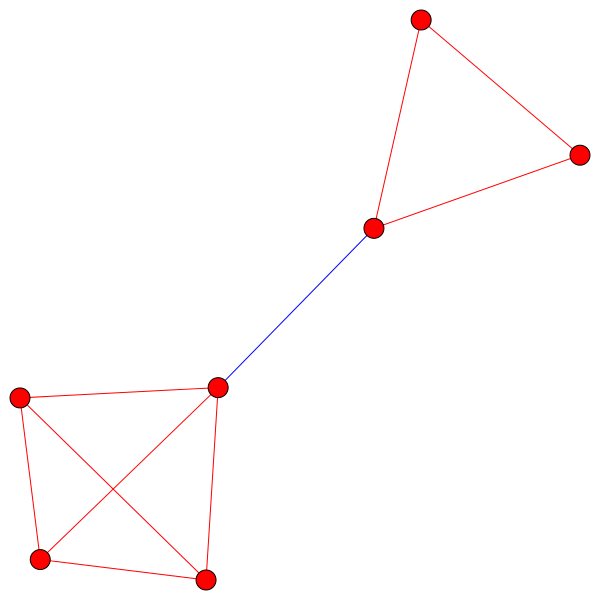
\includegraphics[width=0.60\textwidth]{pic_tieGraph.png}
  \end{center}
  \caption{Ein Graph mit Strong(Rot)- und Weak(Blau) Ties}
  \label{pic_ties}
\end{figure}

 

\section{Modellierung der Verhaltensausbreitung}
\label{s_verhaltenmodel}
Nachdem die grundlegenden Bedingungen für die Modellierung eines sozialen Netzwerkes durch die Verwendung von klar definierten Graphen erfüllt sind, muss nun ein Modell gefunden werden, welches es erlaubt auf den genannten Graphen eine Verhaltensausbreitung zu simulieren. Easly und Kleinberg stellen in ihrem Buch "`Networks, Crowds and Markets"' ein gutes Modell zur Verhaltensausbreitung vor, auf dessen Ausarbeitung das folgende Kapitel maßgeblich aufbaut \cite{Easly10}.
\subsection{Networked Coordination Game}
Die Annahme der Verhaltensausbreitung besteht darin, dass jedes Individuum von der Adaption seines momentanen Verhaltens einen gewissen Nutzen hat. Dieser lässt sich, unter Umständen abstrahiert, beziffern. Nun stellt sich ihm die Möglichkeit ein neues Verhalten anzunehmen, welches einen höheren Wert und somit einen klaren Vorteil gegenüber einem alten Verhalten besitzt. Die Grundzüge dieser Idee spiegeln sich wieder in einem sogenannten "Networked Coordination Game". Hierbei haben die Spieler die Möglichkeit, sich aus einer Auswahl an vorhandenen Verhalten ein beliebiges auszusuchen. Jedes Verhalten besitzt einen eigenen sogenannten Payoff, welcher mit dem Nutzen übersetzt werden kann, welches dieses Verhalten für das Individuum bringt. Unter allein dieser Annahme wäre das Spiel schnell zu Ende, da sich jeder Spieler automatisch für das Verhalten mit dem höchsten Payoff entscheiden würde. Dies würde jedoch nicht den komplexen Verbindungen zwischen den Personen innerhalb eines Netzwerks Rechnung tragen. Daher muss eine Möglichkeit implementiert werden, dass die Payoffs eines Verhaltens abhängig sind von dem der unmittelbaren Nachbarn.\\\\ Die Darstellung der Payoffs in einer sogenannten "Payoff-Matrix" hilft dabei, die Idee zu veranschaulichen, dass der Nutzen eines Verhaltens auch davon abhängt, was ein benachbarter Mitspieler als sein Verhalten gewählt hat. Tabelle \ref{my-label} stellt die Payoff-Matrix dar, welche als Grundlage für die Verhaltensausbreitung dient. Die hier definierte Funktion $p$ legt fest, was für einen Payoff Spieler eins und Spieler zwei beim Auswählen ihrer Verhalten beziehen. Sollten sich beide Spieler für das gleiche Verhalten entscheiden, so erhalten sie den jeweiligen Payoff. Bei einer heterogenen Entscheidung gibt es keine Punkte. Hiermit soll der Eigenschaft Rechnung getragen werden, dass wir stets einen Vorteil haben unser Verhalten dem unserer unmittelbaren Nachbarn anzupassen. Verwenden zwei benachbarte Personen inkompatible Verhalten, profitieren sie nicht voneinander.
\begin{table}[h]
\centering
\caption{Exemplarische Payoff-Matrix}
\label{my-label}
\begin{tabular}{|l|l|l|l|}
\hline
                           & \multicolumn{3}{l|}{Spieler 1}          \\ \hline
\multirow{3}{*}{Spieler 2} &             & Verhalten A & Verhalten B \\ \cline{2-4} 
                           & Verhalten A & p(a,a)      & p(0,0)      \\ \cline{2-4} 
                           & Verhalten B & p(0,0)      & p(b,b)      \\ \hline
\end{tabular}
\end{table}
Diese Payoff Matrix besitzt ebenfalls zwei sogenannte Nash-Equilibria (benannt nach dem Mathematiker John Nash) in den Fällen, dass beide Spieler sich für identische Verhalten entschieden haben. Per Definition des Nash-Equilibriums kann sich, ausgehend von diesen Situationen kein Spieler einen weiteren Vorteil verschaffen, indem er allein sein Verhalten ändert.\\\\
Unter diesen Voraussetzungen wird jedoch noch nicht berücksichtigt, dass es in einem sozialen Netzwerk nicht nur Pärchen gibt, sondern ein Individuum sein Verhalten mit unter Umständen deutlich mehr Nachbarn abstimmen muss. Was bedeutet, dass in eine Kostenrechnung, die das bessere Verhalten auswählt, nicht nur allein die Payoffs ausschlaggebend sein dürfen. Auch die Anzahl der Nachbarn welche entweder das eine oder das andere Verhalten bereits adaptiert haben muss berücksichtigt werden.

 % 
 \begin{equation}
 \label{formel_payoffA}
 P_a = p*a*d
 \end{equation}
 %
  % 
 \begin{equation}
 \label{formel_payoffB}
 P_b = (1-p)*b*d
 \end{equation}
 %
Formel \ref{formel_payoffA} zeigt die Berechnung des Payoffs $P_a$, welchen ein Individuum erhalten würde wenn es insgesamt $d$ Nachbarn besitzt und der Bruchteil $p$ davon sich bereits für das Verhalten A entschlossen hat. Formel \ref{formel_payoffB} ist äquivalent ausgelegt für den Payoff $P_b$. Hier wird davon ausgegangen, dass es nur zwei unterschiedliche Verhalten A und B zur Auswahl gibt und jedes Individuum zwangsweise eines der beiden adaptiert haben muss. Dies gilt auch für das in obigem Beispiel erwähnte Individuum welches eine Entscheidung trifft. Es selbst kann beispielsweise B oder A adaptiert haben ohne, dass dies seine Entscheidung beeinflusst, da nach Definition in Auflistung \ref{enum_graphConditions} Niemand als sein eigener Nachbar zählt.
 %
  \begin{equation}
 \label{formel_payoffCompare}
 p*a*d \geq (1-p)*b*d
 \end{equation}
 %
Verhalten A wäre folglich die bessere Wahl, wenn Formel \ref{formel_payoffCompare} erfüllt ist. Dabei gehen wir hier und in allen folgenden Beispielen davon aus, dass geprüft wird ob ein initial auf B gepoltes Netzwerk, einen Wechsel hin zu Verhalten A vollziehen kann. Unter dieser Annahme wird dem Verhalten A auch der Vorteil gegeben, dass bei einem Gleichstand der beiden Payoffs $P_a$ und $P_b$ das Verhalten A adaptiert wird.
%
  \begin{equation}
 \label{formel_payoffFraction}
 p \geq \frac{b}{a+b}
 \end{equation}
 %
Formel \ref{formel_payoffFraction} erhält man durch Umformulierung der Formel \ref{formel_payoffCompare} und kann somit die Aussage treffen, dass wenn ein $p$ Bruchteil der Nachbarn eines Individuums das Verhalten A adaptiert haben, diese Person ebenfalls zu Verhalten A wechseln wird. Die rechte Seite der Formel \ref{formel_payoffFraction} wird als Threshold bezeichnet und im weiteren Verlauf mit $q$ adressiert. Der Threshold ist, im homogenen Fall, für das gesamte Netzwerk identisch. Er beschreibt den Bruchteil an Nachbarn welche, abhängig von den Payoffs $a$ und $b$ mindestens nötig sind, um ein Individuum zur Adaption von Verhalten A zu bewegen.

\subsubsection{Heterogener Threshold}
\label{sss_heteroThresh}
Die Vorstellung, dass alle Personen innerhalb eines sozialen Netzwerks den gleichen Threshold besitzen, ist künstlich ideal und für eine einfache Analyse sehr dankbar, entspricht jedoch nur unzureichend der Realität. Unter dieser Bedingung könnte man beispielhaft davon ausgehen, dass wenn $50\%$ der Nachbarn eines Individuums Verhalten A adaptiert haben, wird diese Person ebenfalls wechseln. Allerdings ist jeder Mensch verschieden und besitzt somit seinen ganz individuellen Threshold. Manche lassen sich leichter beeinflussen und es genügen schon $30\%$ der Nachbarn um sie zum Wechseln zu bringen. Andere sind hartnäckiger und benötigen den Zuspruch von $80\%$ ihrer Nachbarn um alte Gewohnheiten aufzugeben. Diesen Umstand repräsentiert das hier vorgestellte Modell der Verhaltensausbreitung, mit der Möglichkeit heterogene Thresholds zu verwenden.\\\\
Bei der Anwendung von heterogenen Thresholds besitzt nun jeder Spieler einen ganz eigenen Payoff für die beiden zur Verfügung stehenden Verhalten. Dies spiegelt sich auch in der Payoff Matrix für den Fall eines Networked Coordination Game mit heterogenen Thresholds wieder(Tabelle \ref{table_payofHetero}).
\begin{table}[h]
\centering
\caption{Payoff Matrix mit heterogenen Thresholds}
\label{table_payofHetero}
\begin{tabular}{|l|l|l|l|}
\hline
                           & \multicolumn{3}{l|}{Spieler 1}           \\ \hline
\multirow{3}{*}{Spieler 2} &             & Verhalten A  & Verhalten B \\ \cline{2-4} 
                           & Verhalten A & p($a_1$,$a_2$) & p(0,0)      \\ \cline{2-4} 
                           & Verhalten B & p(0,0)       & p($b_1$,$b_2$)      \\ \hline
\end{tabular}
\end{table}
Somit besitzt jeder Knoten $k$ seinen individuellen Threshold $q_k$ dargestellt in Formel \ref{formel_thresholdHetero}.

%
  \begin{equation}
 \label{formel_thresholdHetero}
 q_k =  \frac{b_k}{a_k+b_k}
 \end{equation}
 %
 
\subsubsection{Beispiel mit homogenen Thresholds}
\label{sss_beispielHomo}
In Abbildung \ref{pic_cascade} ist der Ablauf einer Verhaltensausbreitung in einem Netzwerk mit 10 Knoten sichtbar. Als Ausgangssituation ist das gesamte Netzwerk auf Verhalten B eingespielt (rot markiert). Ausgehend von einem zufällig gewählten initialen Adopter, unter Berücksichtigung der Payoffs $a=2$ und $b=1$, kann für jeden Schritt separat nachvollzogen werden, warum die einzelnen Knoten von Rot auf Grün gewechselt haben.\\\\
\begin{figure}
  \begin{center}
    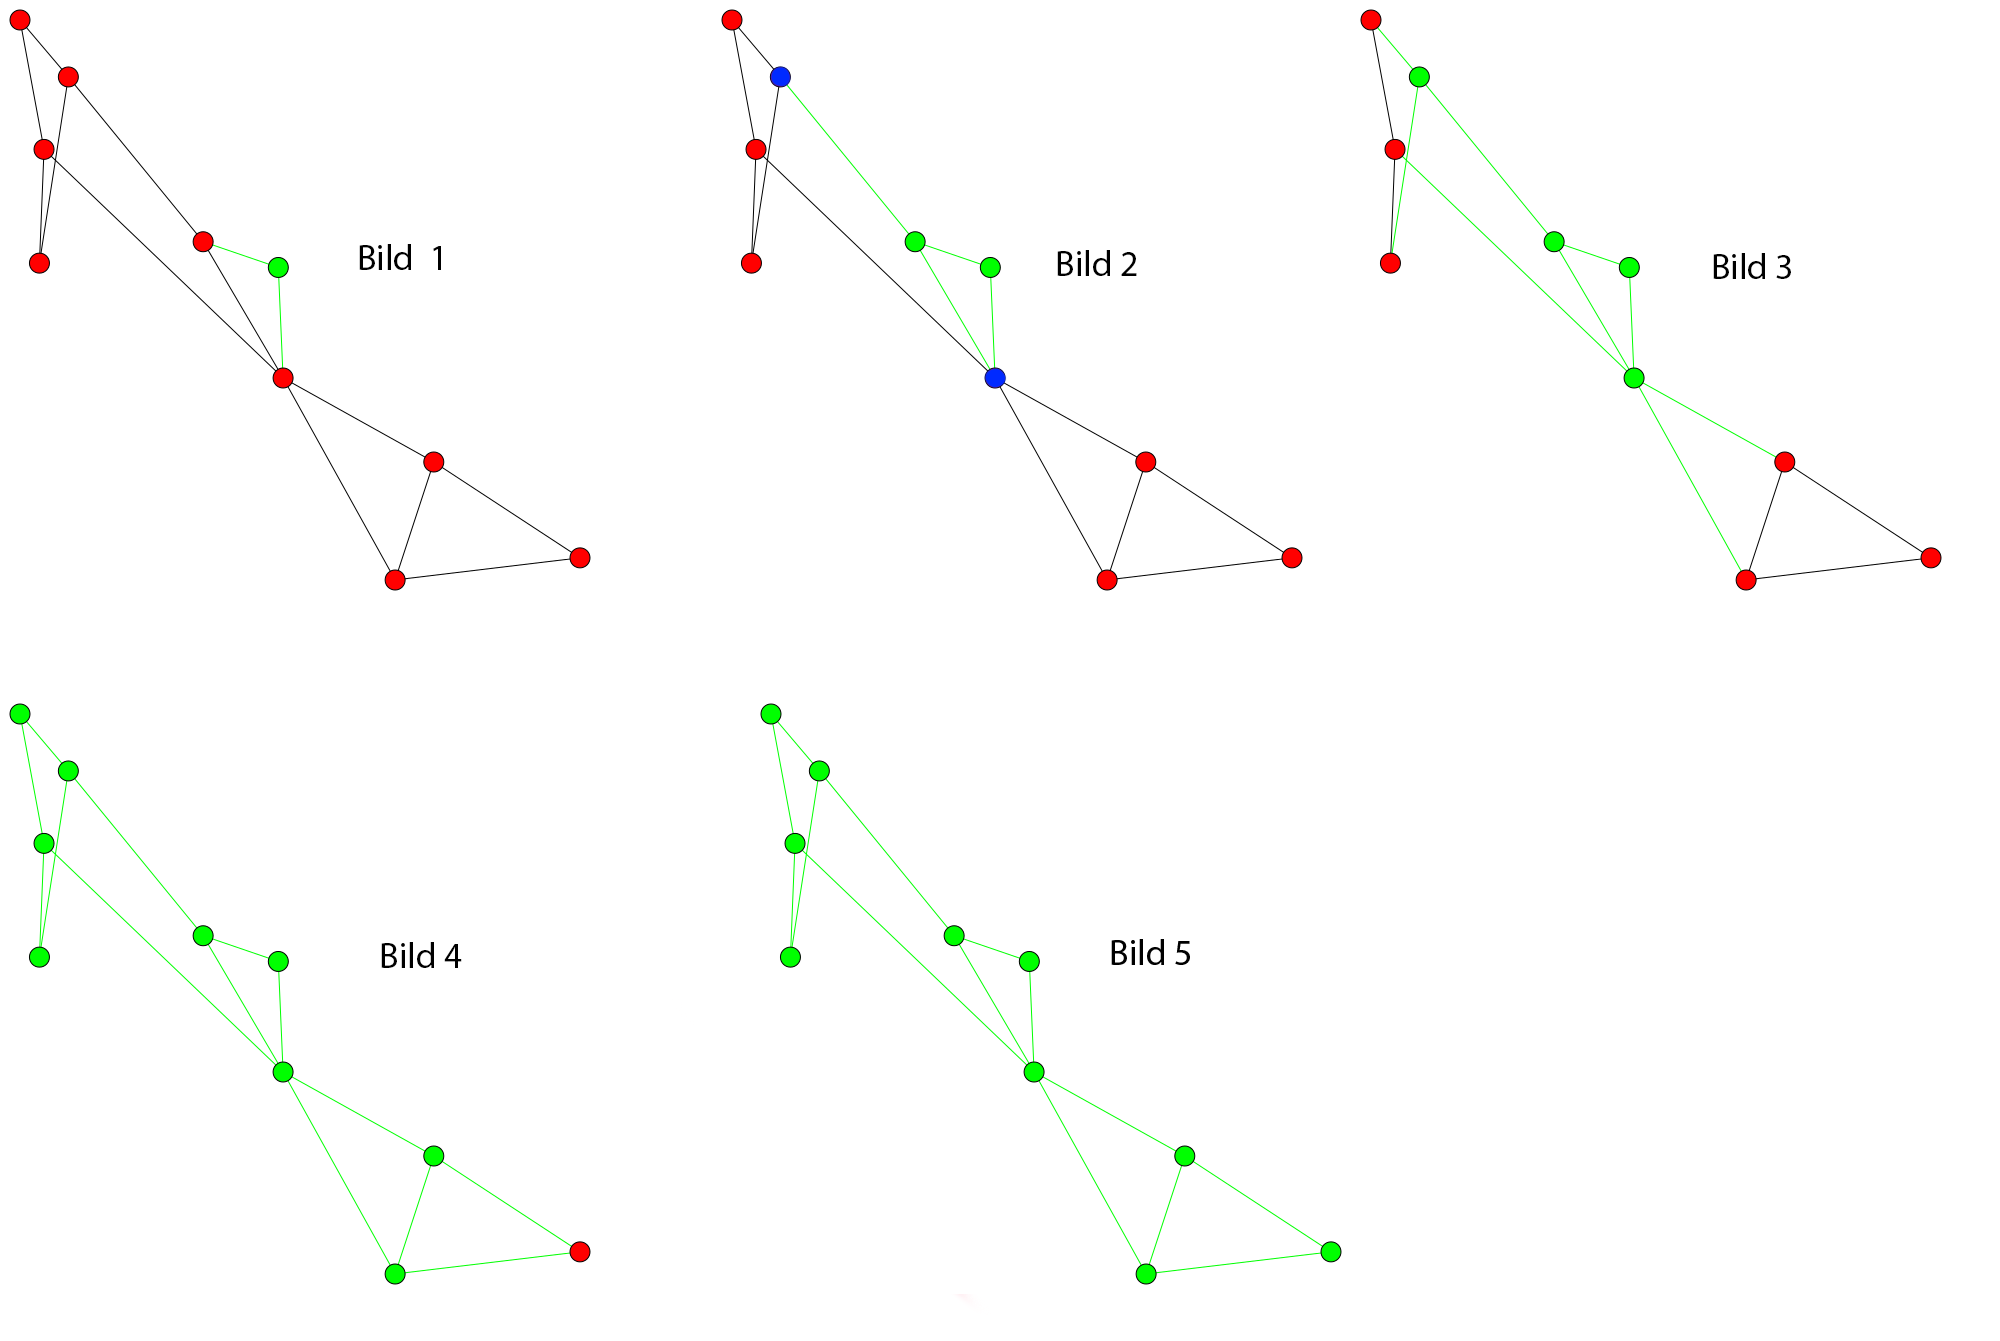
\includegraphics[scale=0.2]{pic_cascade.png}
  \end{center}
  \caption{Ausbreitung der Beispielkaskade}
  \label{pic_cascade}
\end{figure}Beispielhaft wird dies anhand des Steps Bild 2 zu Bild 3 beschrieben. In Bild 2 sind lediglich zwei (grüne) Knoten bisher auf das neue Verhalten $A$ gewechselt. Die hier blau markierten Knoten sind mögliche Kandidaten, welche bis zum nächsten Step wechseln könnten. Den oberen Knoten betrachtend ist ersichtlich, dass er insgesamt über 3 Nachbarn verfügt. Einer davon hat sein Verhalten bereits zu $A$ gewechselt, was ausreicht um den $\frac{1}{3}$ Threshold zu erfüllen. Ähnliches zeigt sich anhand des unteren blauen Knotens. Dieser hat insgesamt 5 Nachbarn, von welchen zwei Verhalten $A$ verwenden. Da $\frac{2}{5} > \frac{1}{3}$ ist der benötigte Threshold mehr als erfüllt. Beide Knoten wechseln im Step zu Bild 3 auf das neue Verhalten $A$. Analog lässt sich die weitere Verbreitung des Verhaltens $A$ durch das Netzwerk verfolgen.

\subsection{Definition einer Kaskade}
Die im Kapitel \ref{sss_beispielHomo} zu beobachtende Kettenreaktion, wird im Rahmen der Verhaltensausbreitung als Kaskade bezeichnet. Der Begriff ursprünglich aus dem Französischen stammend ("`cascade"' - Wasserfall), wird auch im Deutschen verwendet, bei der Beschreibung von über mehrere Stufen abfallenden Wasserfällen. Diese Interpretation lässt sich nun direkt auf die Verhaltensausbreitung übertragen, wo auch in mehreren Stufen (Steps) sich ein Verhalten immer weiter ausbreitet. Allgemein lässt sich von einer Kaskade sprechen, wenn in einem Netzwerk, welches den zuvor festgelegten Definitionen genügt, ausgehend von einem kleinen Kreis initialer Innovatoren, ein neues Verhalten nach und nach das gesamte Netzwerk erobert. Ist das Ergebnis absolut, also zum einem Endzeitpunkt $t_n$ einer Kaskade verwendet jeder Knoten das von ihr verbreitete Verhalten, spricht man von einer vollständigen Kaskade.
\subsection{Cluster als natürliche Hindernisse}
\label{ss_cluster}
Wie im vorherigen Kapitel bereits angesprochen wurde, ist es nicht garantiert, dass ausgehend von den initialen Innovatoren, eine vollständige Kaskade entsteht. Gewisse Strukturen eines sozialen Netzwerks können die Ausbreitung einer Kaskade zum Stillstand bringen, gänzlich unabhängig von der Zeit (oder der Anzahl an Steps). Diese Strukturen werden Cluster genannt. Ein Cluster besteht aus einem Zusammenschluss von mehreren, eng verknüpften Knoten. Diese bilden ein verwobenes Geflecht, welches von innen her alle seine Mitglieder stark genug beeinflusst, um eine Einflussnahme von Außen völlig auszuschließen.\\\\
Easley und Kleinberg \cite{Easly10} definieren einen Cluster wie folgt: \emph{Ein Cluster ist ein Zusammenschluss von Knoten innerhalb eines Graphen. Wenn für jeden Knoten innerhalb eines Clusters gilt, dass ein $x$-Bruchteil seiner Nachbarn sich ebenfalls innerhalb des Clusters befinden, so besitzt der Cluster die Dichte $x$}. Veranschaulichend lässt sich festhalten, dass die Menge aller Knoten eines Graphen
ebenfalls einen Cluster der Dichte $1$ bildet. Ersichtlich ist dies anhand von Abbildung \ref{pic_ties}, wo das obere Dreieck einen Cluster der Dichte $\frac{2}{3}$ und das untere Viereck einen Cluster der Dichte $\frac{3}{4}$ bildet.\\\\
Wenn nun eine Kaskade durch ein Netzwerk läuft, welches einen Threshold $q$ besitzt und sich gleichzeitig in diesem Netzwerk ein Cluster mit einer Dichte $x > (1-q)$ befindet, so wird die Kaskade niemals vollständig werden. Da ein Knoten innerhalb des Clusters, gemäß des Thresholds, mindestens $q\%$ Nachbarn mit neuem Verhalten benötigt. Durch die Definition der Dichte des Clusters jedoch $x\%$ der Nachbarn innerhalb des Clusters sind, also selbst noch das alte Verhalten benutzen ohne Chance das neue zu adaptieren. Somit können die Knoten außerhalb des Clusters niemals die nötige Mehrheit erlangen, um den Knoten innerhalb zum Umschwenken zu bewegen. \\\\
Cluster sind folglich die natürlichen und auch einzigen Hindernisse von Kaskaden. Gelingt es einer Kaskade nicht ein Netzwerk vollständig zum Umschwenken zu bewegen, dann lässt sich direkt daraus schließen, dass dieses Netzwerk einen Cluster mit der Dichte $x > (1-q)$ enthält.

\subsubsection{Cluster mit heterogenen Thresholds}
In Kapitel \ref{sss_heteroThresh} wurde bereits eine Erweiterung des Modells vorgestellt, bei welcher die Knoten nicht mehr einen einheitlichen globalen Threshold besitzen. Stattdessen hat jeder Knoten einen individuellen Threshold. Die Definition der Dichte eines Clusters im vorherigen Abschnitt bezog sich jedoch unmittelbar auf einen global einheitlichen Threshold. Um Cluster nun für Netzwerke definieren zu können, welche heterogene Thresholds besitzen muss ein neuer Begriff eingeführt werden. Unter einem "`Blocking Cluster"' versteht man eine Ansammlung von Knoten mit heterogenen Thresholds, von denen alle ihre jeweilig individuelle Bedingung zur Dichte eines Clusters erfüllen. Das bedeutet, dass drei Knoten $X, U$ und $W$ alle unterschiedliche Thresholds besitzen und doch zusammen einen Blocking Cluster bilden. Genau dann wenn für jeden individuellen Threshold die Bedingung erfüllt ist, dass sich mehr als $(1-q_x)\%$\footnote{Equivalent für $1-q_u$ und $1-q_w$} der Nachbarn innerhalb des Blocking Clusters befinden.
 
\subsection{Kapazität einer Kaskade}
Der Threshold eines Netzwerkes ist, ersichtlich aus Formel \ref{formel_payoffFraction} abhängig von den beiden Payoffs $a$ und $b$. Um den Threshold $q$ abzusenken, um beispielsweise das dichte Netz eines Clusters vielleicht doch durchdringen zu können, bieten die beiden Werte $a$ und $b$ einen gewissen Spielraum. Jedoch ausgehend von der Annahme, dass man bestrebt ist das Verhalten $A$ innerhalb eines Netzwerks zu verbreiten, verringert sich dieser Spielraum lediglich noch auf den Faktor $a$ (da man keinen Einfluss auf das vorherrschende Verhalten $B$ hat). Dieser Faktor $a$ muss erhöht werden um ein Absinken des Thresholds zu bewirken. Angewandt auf die Realität könnte dies bedeuten, dass eine Firma ihr Produkt mit weiteren Investitionen verbessert um seine Qualität zu erhöhen und damit den Payoff zu steigern. Allerdings besteht hierbei die Gefahr, dass man zu viel investiert und das Produkt sich vielleicht auch mit einem niedrigeren Payoff und weniger kostspieligen Investitionen am Markt durchgesetzt hätte.\\
An diesem Punkt wird die sogenannte Kapazität einer Kaskade interessant. Diese ist eine gegebene Eigenschaft eines jeden individuellen Netzwerks und wird definiert durch den höchst möglichen Threshold q (und damit verbunden dem kleinsten Payoff a) für welchen eine Kaskade ein Netzwerk vollständig umstimmen kann.\\\\
Um dies korrekt analysieren zu können, müssen zunächst weitere Bedingungen für den Graphen angenommen werden. Die Auswahl der Innovatoren muss so gewählt werden, dass ihre Anzahl stets deutlich kleiner ist als die gesamte Anzahl an Knoten. Bei der Betrachtung eines Netzwerks mit $100$ Knoten von denen $90$ Innovatoren sind, würde man kaum relevante Ergebnisse bezüglich der Verhaltensausbreitung beobachten können. Für den allgemeinen Fall legt man deswegen für das Netzwerk fest:
\begin{enumerate}
\item Das Netzwerk besteht aus unendlich vielen Knoten.
\item Jeder Knoten hat nur endlich viele Nachbarn.
\item Die Anzahl $I_0$ der Innovatoren ist endlich. Hierdurch ist die Bedingung der kleinen Anzahl an Innovatoren gegeben. Gegenüber einer unendlichen Zahl von Knoten ist eine endliche Anzahl an Pionieren immer ausreichend klein.
\end{enumerate}
Alle zuvor festgelegten Bedingungen für den Graphen gelten auch weiterhin. Damit ist die Grundlage für die Analyse der Kapazität einer Kaskade gestellt.
\subsubsection{Kapazität des infiniten Pfades}
\label{sss_kapinfinit}
Eine der einfachsten Netzwerkstrukturen ist der infinite Pfad, eine eindimensionale Kette von Knoten, welche sich von einem Startpunkt aus in beide Richtungen unendlich ausbreitet. Trotz der unendlichen Ausdehnung genügt bereits ein einzelner Innovator $v_i$ um die Kapazität dieses Netzwerks zu demonstrieren. Zudem ist die Bewegung der Kaskade nach links und rechts entlang des Pfades, ausgehend von $v_i$, identisch. Somit genügt es vollkommen nur eine Seite zu betrachten.\\
Ausgehend von einem beispielhaften Threshold von $30\%$ würde sich die Kaskade vollständig ausbreiten da für die unmittelbaren Nachbarn von $v_i$ die Bedingung des Thresholds mehr als erfüllt ist ($50\% > 30\%$). Allerdings wäre diese Ausbreitung vielleicht auch mit einem höheren Threshold und niedrigerem Payoff $a$ möglich gewesen. Es ist an dieser Stelle nun trivial ersichtlich, dass die Kapazität der Kaskade eines infiniten Pfades $\frac{1}{2}$ beträgt. Für größere Threshold Werte wird die Kaskade niemals über $v_i$ hinaus Verbreitung finden. Allerdings gilt die Kapazität $\frac{1}{2}$ natürlich nicht für alle Netzwerke. Das infinite Gitter beispielsweise besitzt die Kapazität $\frac{3}{8}$. Die Kapazität des infiniten Pfades stellt jedoch einen Sonderfall dar. Denn dieser Wert ($\frac{1}{2}$) ist die maximal mögliche Kapazität einer Kaskade, für ein Netzwerk das allen bisher gestellten Bedingungen gerecht wird. Den Beweis hierzu liefern Easly und Kleinberg \cite{Easly10} durch schlüssige Demonstration, dass eine initial endliche Menge an potentiellen Wechselkandidaten für einen Threshold $q > 1/2$ mit jedem weiteren Step stetig kleiner wird. Da das Netzwerk ans ich jedoch unendlich ist, wird der Ausbreitungsprozess unweigerlich zum Stehen kommen, bevor er vollständig ist.

\subsection{Bilinguale Option}
Wenngleich es natürlich das oberste Ziel der Verhaltensausbreitung ist, eine vollständige Kaskade zu erzeugen, so ist dieser Ausgang unter halbwegs realistischen Bedingungen doch eher selten. Meist stellt sich ab einem gewissen Punkt der Ausbreitung einer Kaskade ein Gleichgewicht zwischen den beiden Verhalten ein, in dem beide koexistieren.\\\\
Ein gutes Beispiel hierfür ist die Ausbreitung von Sprachen in Ländern. Die Deutschen sprechen Deutsch und die Franzosen sprechen Französisch. An diesem Zustand wird sich nicht einfach zufällig etwas ändern, sprich der deutschen Sprache wird nie die Ausbreitung in den Cluster Frankreich gelingen und vice versa. Allerdings lässt sich nun an den Grenzen zwischen den beiden Verhalten (oder den beiden Ländern) das Phänomen der bilingualen Option beobachten. Viele Menschen in Luxemburg sprechen weder ausschließlich Deutsch noch Französisch. Stattdessen haben sie sich für eine dritte Möglichkeit entschlossen, beide Sprachen zu sprechen, um bei der Kommunikation einen Vorteil mit beiden Nachbarn zu haben.
\begin{table}[h]
\centering
\caption{Payoff Matrix mit bilingualer Option}
\label{table_payoffBi}
\begin{tabular}{|l|l|l|l|l|}
\hline
                           & \multicolumn{4}{l|}{Spieler A}                                          \\ \hline
\multirow{4}{*}{Spieler B} &    & A     & B     & AB                                                 \\ \cline{2-5} 
                           & A  & $(a,a)$ & $(0,0)$ & $(a,a)$                                              \\ \cline{2-5} 
                           & B  & $(0,0)$ & $(b,b)$ & $(b,b)$                                              \\ \cline{2-5} 
                           & AB & $(a,a)$ & $(b,b)$ & $((a,b)^+$, $(a,b)^+)$ \\ \hline
\end{tabular}
\end{table}
Diese zusätzlich Option lässt sich in der Payoff Matrix (Tabelle \ref{table_payoffBi}) auslesen. Hieraus ist ersichtlich, dass ein Individuum mit adaptiertem Verhalten $AB$ von beiden Verhalten bei seinen Nachbarn profitiert. Die Notation $(a,b)^+$ für den Fall eines Nachbarn welcher ebenfalls $AB$ adaptiert hat, bedeutet, dass in diesem Fall der höhere Payoff von beiden genommen wird.\\
Diese Tatsache erweckt den Eindruck, dass die Adaption von Verhalten AB einen eklatanten Vorteil vor seinen atomaren Varianten A und B hat. Dabei wird jedoch noch nicht das Problem berücksichtigt, dass die Adaption eines Verhaltens AB natürlich einen Mehraufwand für das Individuum mit sich bringt. Es muss nicht nur eine Sprache beherrscht werden sondern zwei. Dieser Fakt muss in die Berechnung eines endgültigen Payoffs mit einfließen. Dazu wird der Malus $c$ definiert. Der Payoff $P_AB$ für Verhalten AB eines Individuums auf dem infiniten Pfad dessen linker Nachbar $A$ sowie rechter Nachbar $B$ adaptiert haben berechnet sich durch Formel \ref{formel_bilingualAB}.
%
  \begin{equation}
 \label{formel_bilingualAB}
 P_{AB} = a + b - c
 \end{equation}
 %
Während das Modell im Fall ohne bilinguale Option noch lediglich zwischen zwei Ergebnissen unterschied \footnote{Die Kaskade schafft es ein Netzwerk vollständig umzudrehen oder nicht.}, müssen mit der zusätzlichen Option weitere Fälle unterschieden werden.
\begin{figure}
  \begin{center}
    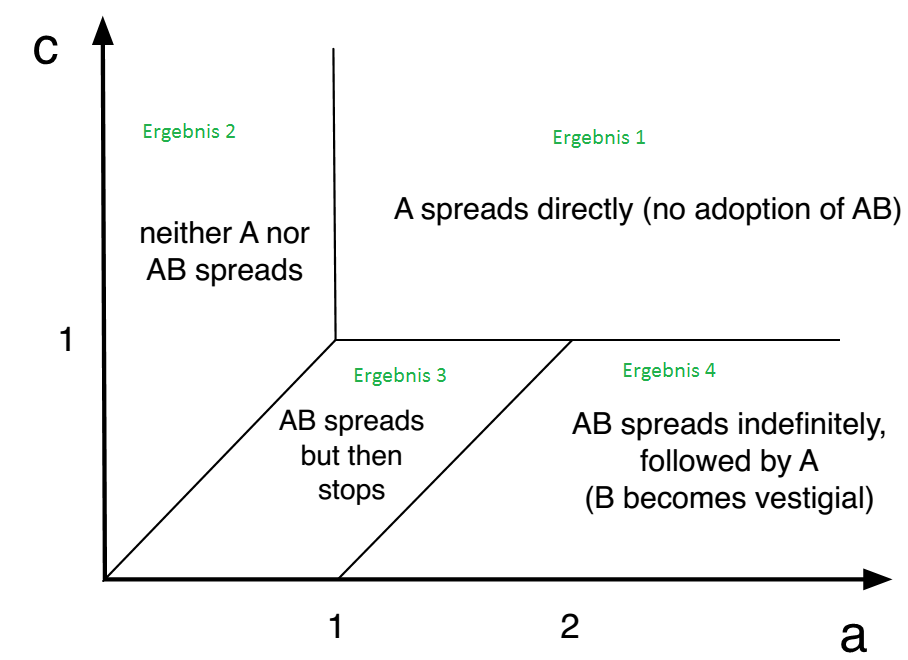
\includegraphics[scale=0.7]{bilingual.png}
      \caption{Mögliche Ergebnisse der bilingualen Option in 2D}
      Quelle: Easly und Kleinberg \cite{Easly10}
        \label{pic_bilingual}
  \end{center}


\end{figure}In Abbildung \ref{pic_bilingual} lassen sich, abhängig von den Werten des Payoffs $a$ und des Malus $c$, vier mögliche Ergebnisse für den Fall des infiniten Pfades definieren.  Ergebnis 1 und 2 sind die Standardfälle welche schon aus dem ursprünglichen Modell bekannt sind. Entweder $A$ breitet sich vollständig aus oder überhaupt nicht. Ergebnis 4 kann im Endeffekt auch als eine vollständige Ausbreitung von $A$ interpretiert werden, jedoch schiebt diese stets eine Welle aus $AB$ vor sich her. Interessant ist besonders Ergebnis 3 da in diesem Fall lediglich eine einzelne Ausbreitung von $AB$ stattfindet und die Kaskade dann anhält. Dieser durch Ergebnis 3 entstehende Knick im Bereich der Ausbreitung von $A$ kann interpretiert werden, dass gerade ein mittelmäßiger Wert für den Malus $c$ sich negativ auf die Ausbreitung einer Kaskade auswirkt.



\section{Virales Marketing}
Wenngleich auch die bisher vorgestellten Konzepte der Verhaltensausbreitung aus einer rein wissenschaftlichen Perspektive bereits interessant sind, so ergibt sich das wesentliche Interesse aus dem Bereich des Marketings. Über die Jahrhunderte hinweg wurden zahlreiche Methoden entwickelt, mit denen Produzenten von Gütern oder Dienstleistungen die mögliche Käuferschaft auf ihr Produkt aufmerksam machen wollten. Diese reichen von klassischer Werbung (TV, Plakat, etc.) über kleine Geschenke bis zu aufwändig produzierten Veranstaltungen oder Sponsorings.\\ Eine sehr neue Variante ist dabei das sogenannte Viral Marketing. Dieses ist, bei dem Versuch einen Vergleich mit früheren Methoden herzustellen, noch am ehesten mit der klassischen Mundpropaganda verwandt. Es nutzt den bereits ausführlich in Kapitel 2 besprochenen Umstand, dass Menschen den Empfehlungen oder Verhalten ihrer Freunde und nahen Bekannten mehr Gewicht geben, als dem von einem unbekannten Vertreter an der Haustüre. Letzterer hat für einen potentiellen Kunden stets den fahlen Beigeschmack, dass er selbstverständlich sein Produkt in alle Höhen loben wird um es zu verkaufen. Kommt diese Empfehlung jedoch von einem Freund der keinen finanziellen Gewinn damit hat, wirkt sie sofort ehrlicher und somit nachhaltiger.\\
Diesen Umstand respektierend, wird Virales Marketing dahingehend konstruiert, dass für jeden der davon erreicht wird der Eindruck suggeriert wird, die Empfehlung käme von einem Freund. Beispielsweise könnte ein Post auf dem sozialen Netzwerk Facebook, welcher sich mit den Vorteilen eines neuen Web Browsers beschäftigt, von einer Person A ein Like bekommen. Dieses Like wird sofort allen Freunden von A angezeigt und macht diese direkt darauf aufmerksam. Vielleicht geben sie nun auch alle dem Post ein Like und so breitet sich die Nachricht von einem neuen Web Browser viral innerhalb des Netzwerks aus. Das alles mit verschwindenden Kosten für denjenigen welcher initial den Post verfasst hatte. \cite{mindcomet08}
\subsection{Change Agents}
Nun wurde im eben genannten Beispiel noch die Idee vertreten, dass der initiale Zündfunke (der Post auf Facebook) von einem Vertreter der Interessengruppe selbst kommt. Nur die Verweise darauf kommen dann von Freunden und Bekannten. Um den Effekt des Viralen Marketings noch zu verstärken kann auch schon der initiale Post von einem Menschen kommen der nicht direkt ersichtlich mit der werbenden Firma zu tun hat. Diese Personen, welche heutzutage gerne als Idole oder Trendsetter bezeichnet werden, sind im Umfeld der Verhaltensausbreitung nichts anderes als gekaufte Quasi-Innovatoren. Gerne nutzen Firmen hierfür Prominente die in den sozialen Medien sehr präsent sind. Beispielsweise besitzt die Künstlerin Kate Perry über 70 Millionen Follower auf dem online Netzwerk Twitter (Stand 2015). Sie ist somit ein äußerst begehrter Change Agent für eine gewisse Zielgruppe, da sie mit einer einzelnen Nachricht eine riesige Fangemeinde erreichen kann. Eine Fangemeinde aus leicht beeinflussbaren Menschen welche ihrem Idol nur zu gerne nacheifern, wenn es eine neue Schuhmarke als besonders angesagt verkündet. Das anwerben von Change Agents wird auch gerne im Zusammenhang mit Clustern genannt. Gerade um diese eng verflochtenen Strukturen zu durchdringen könnte eine Firma entweder ihr Produkt derart qualitativ hochwertig machen um den Threshold weit genug zu drücken. Dies ist jedoch unter Umständen mit hohen Kosten verbunden. Alternativ ist es möglicherweise billiger einen einflussreichen Menschen innerhalb des Clusters zu kaufen. Dieser würde dann als Change Agent das neue Verhalten von innen in seinem Netzwerk verbreiten was von außen niemals möglich gewesen wäre.
\subsection{Beispiele für Virales Marketing}
Ein besonders erfolgreiches Beispiel für Virales Marketing der letzten Jahre, war die Kampagne von Barack Obama zur Präsidentenwahl im Jahr 2008. Sein Wahlkampfteam setzte hier bereits von Anfang an sehr stark auf die Macht der sozialen Medien, war mit Facebook und Twitter Accounts präsent und stachelte die virale Verbreitung von ikonischen Bildern und Nachrichten an. Am berühmtesten davon ist nach wie vor das stilisierte Abbild von Barack Obama selbst mit dem Schriftzug "`HOPE"'. Dieses wurde millionenfach in den online Netzwerken geteilt, wobei jedes Teilen wieder den bereits besprochenen Effekt hatte: Nicht das Wahlkampfteam von Barack Obama empfohl ihn als Kandidaten, sondern Freunde und Bekannte taten dies.\\\\
Ein weiteres Beispiel welches stets Erwähnung finden muss in Abhandlungen über Virales Marketing ist die perfekt inszenierte Onlinekampagne zum 1999 veröffentlichen Indy-Horror Film "`The Blair Witch Project"'. Dieser mit wackeligen Handkamerabildern gefilmte Streifen, handelte von der Geschichte mehrerer Jugendliche, die in den Wäldern Marylands auf der Suche nach der legendären Blair Witch verschollen sind. Der Film ist ausschließlich mit Handkameras gefilmt und wirkt mehr wie eine wackelige Dokumentation dieser besagten Jugendlichen. Gezielt wurde hier bei der Vermarktung versucht, den Eindruck zu erwecken diese Ereignisse hätten sich tatsächlich zugetragen. Dies geschah durch geschickt platzierte kleine Details auf Webseiten, welche dann in den damaligen Netzwerken und unter Freunden rege Verbreitung fanden. Beispielsweise wurden die Schauspieler des Films auf der Film-Datenbank IMDB als Tot oder Vermisst eingetragen, obwohl dies natürlich nicht der Wahrheit entsprach. Das Ergebnis war ein Einspielergebnis von ungefähr 250 Millionen Dollar dem Produktionskosten von circa 20.000 Dollar gegenüber standen. \cite{www_viral} \cite{www_bw}

\section{Fazit}
Abschließend lässt sich die Erkenntnis gewinnen, dass die Untersuchung von Verhaltensausbreitungen in sozialen Netzwerken besonders in der heutigen Zeit von maßgeblicher Bedeutung ist. Wenngleich sie ihre Ursprünge in ersten Studien Anfang der 40er Jahre des letzten Jahrhunderts hat, bietet der Aufstieg des Internets und der sozialen Medien, besonders im Bezug auf das Virale Marketing, einen kommerziell sehr interessanten Ansatz, sich mit detaillierten Modellen und Theorien zur Verhaltensausbreitung zu beschäftigen.


\begin{thebibliography}{9}

\bibitem{morris98}
  Stephen Morris:
  \emph{Contagion},
  Yale University,
  1998.
 
\bibitem{strang98}
	David Strang, Sarah A. Soule:
	\emph{Diffusion in Organisations},
	Annu. Rev. Sociol., 1998, pp. 265-290.
	
\bibitem{Easly10}
	David Easly, John Kleinberg: 
	\emph{Networks, Crowds and Markets},
	Cambridge University Press, 2010, pp. 561-603.
	
\bibitem{Rogers03}
	Everett M. Rogers: \emph{Diffustion of Innovation}, Fifth
	Edition, Free Press, 2003
	
\bibitem{Ryan43} Bryce Ryan, Neil Gross: \emph{Acceptance and 		    Diffusion of Hybrid Corn Seed in Two Iowa Communities}, Agricultural Experiment Station Iowa State College of Agriculture and Mechanic Arts, 1950

\bibitem{mindcomet08} Mindcomet Corporation: Viral Marketing - Understsanding the concepts and benefits of viral marketing, 2008

\bibitem{www_viral} http://www.prospectmx.com/15-of-the-best-viral-marketing-campaigns/

\bibitem{www_bw} http://mwpdigitalmedia.com/blog/the-blair-witch-project-the-best-viral-marketing-campaign-of-all-time/



 

\end{thebibliography}


\end{document}